\newsavebox{\mintedbox}

\begin{figure}[h]
	\centering
	\begin{lrbox}{\mintedbox}
		\begin{minipage}{0.45\textwidth}
			\jscode{code/blacklisted-modules/foo.js}
		\end{minipage}
	\end{lrbox}
	\subfloat[foo/index.js]{\usebox{\mintedbox}}
	\hfill
	\begin{lrbox}{\mintedbox}
		\begin{minipage}{0.45\textwidth}
			\jscode{code/blacklisted-modules/A.js}
		\end{minipage}
	\end{lrbox}
	\subfloat[A/index.js]{\usebox{\mintedbox}}

	\begin{lrbox}{\mintedbox}
		\begin{minipage}{0.48\textwidth}
			\jscode{code/blacklisted-modules/D.js}
		\end{minipage}
	\end{lrbox}
	\subfloat[D/index.js]{\usebox{\mintedbox}}
	\hfill
	\begin{lrbox}{\mintedbox}
		\begin{minipage}{0.45\textwidth}
			\jsoncode{code/blacklisted-modules/blacklist.json}
		\end{minipage}
	\end{lrbox}
	\subfloat[blacklist.json]{\usebox{\mintedbox}}

	\subfloat{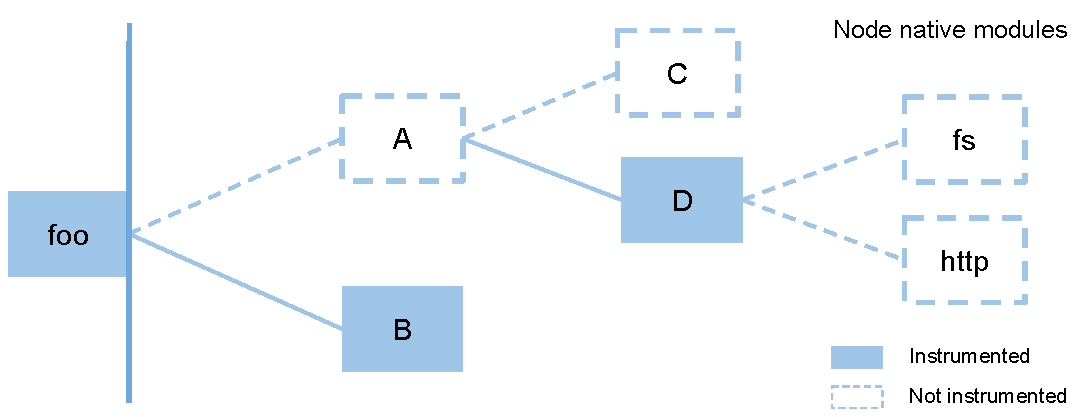
\includegraphics[width=1\textwidth]{figures/approach/blacklisted-modules/blacklisted-modules.pdf}}
	
	\caption[Non-instrumented node modules]{\textbf{Non-instrumented node modules} - Dependencies tree for module \textit{foo}. Modules \textit{A} and \textit{B} are included in the blacklist. Module \textit{D} is instrumented anyway, even though its father is not. Node native modules, like \textit{fs} or \textit{http}, are excluded anyway by Jalangi.}
	\label{fig:blacklisted-modules}
\end{figure}